\documentclass[a4paper,12pt]{article}
\usepackage[slovene]{babel}
\usepackage[utf8]{inputenc}
\usepackage[T1]{fontenc}
\usepackage{lmodern}
\usepackage{amsmath}
\usepackage{hyperref} 
\usepackage{graphicx} 
\usepackage{amsfonts}
\usepackage{eurosym}
\usepackage{stackengine}
\usepackage{fancyhdr}
\usepackage{amssymb}
\usepackage{graphicx}
\usepackage{amsbsy}
\usepackage{mathtools}
\usepackage{amsthm}
\usepackage{graphicx}
\usepackage[output-decimal-marker={,}]{siunitx}

\begin{document}
\title{ Iterativni izračun Nashevega ravnotežja v matričnih igrah}
\author{Eva Babnik}
\date{Maj, 2022}
\maketitle


\newpage
\section{Nashevo ravnotežje in vrednost igre v matričnih igrah}

Spodobi se, da najprej v nekaj stavkih opišem Nashevo ravnotežje ter vrednost igre v matričnih igrah z ničelno vsoto za dva igralca. 
Matrično igro z dvema igralcema lahko predstavimo z matriko izplačil $A=(a_{ij})$, kjer prvi igralec izbere eno izmed $m$ vrstic, drugi pa hkrati izbere enega izmed
$n$ stolpcev. $A_{i\cdot}$ naj označuje $i$-to vrstico, $A_{\cdot j}$ pa $j$ - ti stolpec. Če igralca izbereta $i$-to vrstico in $j$-ti stolpec, potem drugi igralec plača prvemu igralcu $a_{ij}$. \par
Če prvi igralec izbere $i$-to vrstico z verjetnostjo $x_i$ in drugi izbere $j$-ti stolpec z verjetostjo $y_j$, pri čemer velja:
\begin{equation}
    \label{eqn:e1}
    x_i \geq 0,
\end{equation}
\begin{equation}
    \label{eqn:e2}
    \sum x_i = 1,
\end{equation}
\begin{equation}
    \label{eqn:e3}
y_i \geq 0,
\end{equation}
\begin{equation}
    \label{eqn:e4}
    \sum y_i = 1.
\end{equation}
Potem je pričakovano izplačilo prvemu igralcu $\sum \sum a_{ij}x_i y_j$. Poleg tega velja tudi:
\begin{equation*}
    \min_j \sum_i a_{ij}x_i \leq \max_i \sum_j a_{ij} y_j.
\end{equation*}
Trditev o minimaksu nam pove, da za neka vektorja verjetnosti $X = (x_1, \cdots, x_m)$ in $Y = (y_1, \cdots, y_n)$ v zgornji enačbi velja enakost. Tak par $(X^*, Y^*)$
predstavlja optimalno strategijo igre. Vrednost igre $v$ pa je definirana kot:
\begin{equation*}
    v = \min_j \sum_{i} a_{ij}x_i = \max_i \sum_j a_{ij} y_j.
\end{equation*}

Problem matrične igre za dva igralca lahko enostavno rešimo z linearnim programiranjem:
\begin{equation*}
    \begin{split}
    &\min X J_m^T \\
    & \textrm{p. p.} \; XA_j \geq 1, \; \; j = 1, \cdots, n \\
    & X \geq 0
    \end{split}
\end{equation*}
in 
\begin{equation*}
    \begin{split}
    &\max YJ_n \\
    &\textrm{p. p.} \; A_i Y^T \leq 1 \; \; i = 1, \cdots, m\\
    &Y \geq 0,
    \end{split}
\end{equation*}
pri čemer sta $J_m$ in $J_n$ vektorja samih enic primernih velikosti. Algoritem, ki nam z linearnim programiranjem vrne vrednost matrične igre
in optimalno strategijo, sem implemenitrala v funkciji \textit{resitevLP.py}, ki kot vhodni argument sprejme matriko.
\section{Iterativno računanje rešitve igre}
V projektu sem implementirala dva iterativna algoritma, ki nam vrneta optimalno strategijo in vrednost igre ter analizirala kako hitra je konvergenca posameznih metod. 
Za implementacijo sem uporabila programski jezik \textit{Python}, pri analizi metod pa sem si pomagala tudi s programskim jezikom \textit{R}. Celotna koda, ki vsebuje
vse implementacije iterativnih algoritmov, se nahaja v datoteki \textit{projekt.py}, analiza metod pa se nahaja v datoteki \textit{analiza.R} \par

\subsection{Metoda I}

Najprej uvedimo še nekaj nove notacije. Naj velja:
\begin{equation*}
    \begin{split}
    A_i = (a_{1i}, \cdots, a_{mi}, \underbrace{0, \cdots, 0}_{n - \text{komponent}}, -1), \\
    A_{0i} = (\underbrace{1, \cdots, 1}_{m-\text{komponent}}, \underbrace{0, \cdots, 0}_{n-\text{komponent}}, 0) \\
    \text{za} \, \, i = 1, \cdots, n
    \end{split}
\end{equation*} 
in 
\begin{equation*}
    \begin{split}
    A_i = (\underbrace{0, \cdots, 0}_{m - \text{komponent}},-a_{i-n, 1}, \cdots, -a_{i - n, n}, 1), \\
     A_{0i} = (\underbrace{0, \cdots, 0}_{m-\text{komponent}},\underbrace{1, \cdots, 1}_{n-\text{komponent}},  0) \\
    \text{za} \, \, i = n + 1, \cdots, m + n.
    \end{split}
\end{equation*} 
Definirajmo še vektor, ki predstavlja rešitev igre: $Z^* = (X^*, Y^*, v)$. $Z^*$ mora poleg \ref{eqn:e1}, \ref{eqn:e2}, \ref{eqn:e3}, \ref{eqn:e4}, ustrezati še pogoju:
\begin{equation}
\label{eqn:e5}
A_i \cdot Z^* \geq 0 \, \, \text{za} \, \, i = 1, \cdots, m + n.
\end{equation}
Metoda se začne s poljubnim vektorjem $Z^{(1)}$, ki zadošča \ref{eqn:e1}, \ref{eqn:e2}, \ref{eqn:e3} in \ref{eqn:e4}. Sedaj predpostavimo,
 da smo prišli na $k$-ti korak
iteracije, in dobili vektor $Z^{(k)}$,  ki ustreza \ref{eqn:e1}, \ref{eqn:e2}, \ref{eqn:e3} in \ref{eqn:e4}. Če velja tudi
\ref{eqn:e5}, je $Z^{(k)}$ rešitev igre in smo zaključili. Sicer pa naj bo $j_k$ tak indeks, da bo veljalo
$A_{j_k} \cdot Z^{(k)} \leq A_i \cdot Z^{(k)}$ za vse $i = 1, \cdots, m + n$. Če obstaja več takih indeksov, lahko poljubno izberemo.
 Če torej poznamo indeks $j_k$, lahko
dobimo nov vektor $\bar{Z}^{(k+1)} = (\bar{X}^{(k+1)}, \bar{Y}^{(k+1)}, \bar{v}^{(k+1)})$ na sledeči način:
\begin{equation*}
    \bar{Z}^{(k+1)} = Z^{(k)} + \alpha B_{j_k} + \beta B_{0j_k},
\end{equation*}
kjer je
\begin{equation*}
    \alpha = - Z^{(k)} \cdot B_{j_k} [1 - \cos^2{\theta_{j_k}}]^{-1},
\end{equation*}
\begin{equation*}
    \beta = b_{0j_k} - [Z^{(k)} + \alpha B_{j_k}] \cdot B_{0j_k},
\end{equation*}
\begin{equation*}
    b_{0j_k} = \frac{1}{(A_{0j_k}\cdot A_{0j_k})^{1/2}},
\end{equation*}
\begin{equation*}
B_{j_k} = \frac{A_{j_k}}{(A_{j_k} \cdot A_{j_k})^{1/2}}, 
\end{equation*}
\begin{equation*}
B_{0j_k} = \frac{A_{0j_k}}{(A_{0j_k}\cdot A_{0j_k})^{1/2}}
\end{equation*}
in 
\begin{equation*}
 \cos{\theta_{j_k}} = \frac{A_{0j_k} \cdot A_{j_k}}{(A_{0j_k}\cdot A_{0j_k})^{1/2}(A_{j_k}\cdot A_{j_k})^{1/2}}.
\end{equation*}
Sedaj predpostavimo, da velja $j_k < (n +1)$. (V primeru, da bi bil $j_k \geq n + 1$, bi komponente $x$ ostale nespremenjene, postopek, opisan v nadaljevanju, pa bi veljal za $y$ komponente.)
Če $\bar{Z}^{k+1}$ ustreza \ref{eqn:e5}, potem nastavimo $Z^{k+1} = \bar{Z}^{k+1}$,
v nasprotnem primeru pa moramo, da dobimo $Z^{k+1}$, narediti še nekaj korakov. Najprej vse negativne $x$-komponente vektorja $\bar{Z}^{k+1}$ nastavimo na 0.
Predpostavimo, da so $\bar{x}_1^{(k+1)}, \cdots, \bar{x}_r^{(k+1)}, \, \, r < m$ negativne komponente vektorja $\bar{Z}^{(k+1)}$. Nato 
izračunamo vse vsote $\bar{x}_i^{(k+1)} + \frac{\sum_{i=1}^r \bar{x}_i^{(k+1)}}{m - r} $ za $i = r +1, \cdots, m$. Za vsak tak $i$, za katerega
je vsota negativna, nastavimo $x_i^{(k+1)} = 0$. Če nobena vsota ni negativna, lahko tvorimo preostanek vektorja $Z^{(k+1)}$. Spet predpostavimo, da so nekatere vsote za $i = r+1, \cdots, r +s$ negativne. Ponovno izračunamo vsote 
$\bar{x}_i^{(k+1)} + \frac{\sum_{i=1}^{r+s} \bar{x}_i^{(k+1)}}{m - (r+s)} $ za $i = r + s, \cdots, m$. Če nobena vsota ni negativna, tvorimo preostanek vektorja $Z^{(k+1)}$, sicer pa ponavljamo zgornji postopek, dokler nobena od vsot ni negativna.\par
Predpostavimo, da za $i = 1, \cdots, t$ velja, da je $\bar{x}_i^{(k+1)} \leq 0$ ali pa, da je $\bar{x}_i^{(k+1)}$ tak, da je zanj katera od zgoraj definiranih vsot negativna. Potem lahko vektor $Z^{(k+1)}$
tvorimo na sledeči način:
\begin{equation*}
    x_1^{(k+1)} = \cdots = x_t^{(k+1)} = 0,
\end{equation*}  
\begin{equation*}
    x_i^{(k+1)} = \bar{x}^{(k+1)} +  \frac{\sum_{i=1}^{t}\bar{x}_i^{(k+1)}}{m-t} \, \, \text{za} \, \, i = t+1, \cdots, m,
\end{equation*}
\begin{equation*}
    y_j^{(k+1)} = \bar{y}_j^{(k+1)} \, \, \text{za} \, \, j = 1, \cdots, n,
\end{equation*}
\begin{equation*}
    v^{(k+1)} = \bar{v}^{(k+1)}.
\end{equation*}

Opisana metoda je implementirana s funkcijo \textit{iteracija2} in sprejme dva argumenta - \textit{steviloIteracij} in \textit{matrika}. 
Za začetne približke sem vzela
$x_0 = (1 / m, \cdots, 1 / m)$, $y_0 = (1 / n, \cdots, 1 / n)$, $v_0$ pa sem generirala iz enakomerne porazdelitve $U(a,b)$, kjer sta $a$ in $b$ najmanjši in največji 
element matrike po absolutni vrednosti. Funckija \textit{iteracija2} po $k$-iteracijah vrne vektor $Z^{k} = (X^{k}, Y^{k}, v^{k})$, ki predstavlja rešitev igre.

\subsection{Metoda II}
Naslednja metoda, ki sem jo implemenitrala se imenuje statistična Brownova metoda. Temelji na ideji, da so sedanje odločitve odvisne od zgodovine.
1. igralec najprej igra poljubno čisto strategijo $X_{i_1}$, pri čemer je $i_1$ komponenta iz množice $(1, \cdots, m)$ enaka 1, ostale komponente pa so enake 0.
2. igralec nato začne z vektorjem akumulativnih vsot $A^{(1)} = [a_1^{(1)}, \cdots, a_n^{(1)}]$, kjer $A^{(1)}$ predstavlja $i_1$-to vrstico matrike. 2. igralec
nato igra čisto strategijo $Y_{j_1}$, pri čemer je $j_1$ tak indeks iz množice $(1, \cdots, n)$, da velja, da je $a_{j_1}^{(1)}$ najmanjša komponenta vektorja $A^{(1)}$. Če je minimumov več načeloma vzamemo
poljubnega, pri implementaciji pa sem vzela prvi minimum.
1. igralec nato začne z vektorjem akumulativnih vsot $B^{(1)} = [b_1^{(1)}, \cdots, b_m^{(1)}]$, pri čemer je $B^{(1)} \; \; \; j$-ti stolpec matrike.
1. igralec tako uporabi čisto strategijo $X_{i_2}$, pri čemer je $i_2$ tak indeks iz množice $(1, \cdots, m)$, da velja, da je $b_{j_2}^{(1)}$ največja komponenta vektorja $B^{(1)}$
Če je maksimumov več načeloma vzamemo poljubnega, pri implementaciji pa sem vzela prvi maksimum. 1. igralec nato vektorju $A^{(1)}$ prišteje $i_2$ - to vrstico matrike, zatem pa 2. igralec igra na enak način kot prej.
Na $k$-tem koraku imamo vektorja akumulativnih vsot $A^{(k)} = [a_1^{(k)}, \cdots, a_n^{(k)}]$ in $B^{(k)} = [b_1^{(k)}, \cdots, b_m^{(k)}]$. 1. igralec nato igra čisto strategijo $X_{i_k+1}$, pri čemer je $i_{k+1}$ tak indeks, da je $b_{j_k+1}^k$ maksimalna komponenta
vektorja $B^{(k)}$. $A^{(k+1)}$ dobimo tako, da vektorju $A^{(k)}$ prištejemo $j_{(k+1)}$-to vrstico matrike izplačil. 2. igralec tako igra čisto strategijo $Y_{j_(k+1)}$, pri čemer je $j_{(k+1)}$ tak indeks, da je $a^{(k+1)}_{j_(k+1)}$ najmanjša komponenta vektorja $A^{(k+1)}$.
Postopek ponavljamo. Dokazati se da, da zaporedje  $\frac{\sum_{n=1}^k X_{i_n}}{k}$ ali konvergira k optimalni strategiji $X^*$ ali pa ima tako podzaporedje. Prav tako tudi zaporedje  $\frac{\sum_{n=1}^k Y_{i_n}}{k}$ ali konvergira k optimalni strategiji $Y^*$ ali pa ima podzaporedje, ki konvergira.
Vrednost igre pri tem algoritmu dobimo kot $\max_{k = 1, 2, \cdots} \frac{\min_{i \in (1, \cdots, n)} a_i^{(k)}}{k}$ in kot
$\min_{k = 1, 2, \cdots} \frac{\max_{i \in (1, \cdots, m)} b_i^{(k)}}{k}$. \par
Opisana metoda je implementirana s funkcijo \textit{iteracijaBrown} in sprejme 2 argumenta - \textit{matrika} in \textit{steviloIteracij}. Funkcija vrne optimalni strategiji po $k$-tih korakih iteracije $X^{(k)}$ in  $Y^{(k)}$, ter vrednost igre $v^{(k)}$. Za vrednost igre sem vzela povprečje 
$\max_{k = 1, 2, \cdots} \frac{\min_{i \in (1, \cdots, n)} a_i^{(k)}}{k}$ in 
$\min_{k = 1, 2, \cdots} \frac{\max_{i \in (1, \cdots, m)} b_i^{(k)}}{k}$
\section{Analiza konvergence, časovna zahtevnost in rezultati}
Vse meritve sem opravila s prenosnim računalnikom s procesorjem 2.40GHz Intel(R) Core(TM) i5-6300U CPU in 8GB spomina.  
Naj najprej povem, da sem vsak poskus ponovila 10-krat in nato vzela povprečje rezultatov. 
Najprej si bomo pogledali, kako na treh matrikah različnih dimenzij delujejo zgoraj opisani algoritmi. Začnimo
z matriko dimenzije $ 3 \times 2$:
\begin{equation*}
\begin{bmatrix}
    4 & 3\\
    2 & 4\\
    5 & 2
\end{bmatrix}
\end{equation*}

Vrednost prve matrične igre je $v^* = \frac{10}{3}$, medtem, ko je mešano Nahevo ravnovesje $X^* = [\frac{2}{3}, \frac{1}{3}, 0]$ in $Y^* = [\frac{1}{3}, \frac{2}{3}]$. \par
Za začetek si poglejmo graf \ref{fig:vred1}, ki prikazuje, kako hitro konvergira vrednost igre, dobljena z obema metodama proti pravi vrednosti, ki je označena s črno 
črto. Ta in vsi naslednji grafi zaradi boljše preglednosti prikazujejo le prvih 100 korakov iteracije. \\
Na grafu opazimo, da se vrednost igre, dobljene s prvim algoritmom, že po nekaj korakih iteracije popolnoma približa pravi vrednosti, medtem ko je konvergenca pri drugi metodi počasnejša. 
Zanimiv je tudi pojav, da se vrednost pri prvem algoritmu v nekaterih zgodnejših korakih prej približa pravi vrednosti igre, kot v poznejših. To bi lahko pomenilo, da prva metoda ne izbere nujno najbližje rešitve.
\begin{figure}
    \centering
    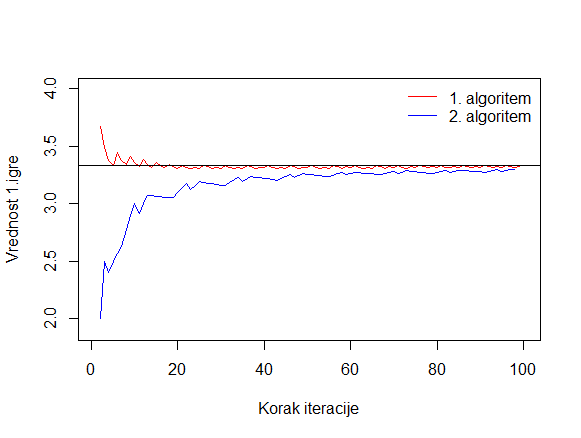
\includegraphics[width=12cm]{1.igra_vred.png}
    \caption{Vrednosti prve matrične igre}
    \label{fig:vred1}
  \end{figure}

  Naslednji graf \ref{fig:napaka1} prikazuje kako se obnaša največja maksimalna napaka, dobljena pri obeh algoritmih v odvisnosti od korakov iteracije.
   Napaka je definirana kot $napaka = ||Z^* - Z^{k}||_{\infty}$. Vidimo, da je napaka najprej največja pri drugem algoritmu, a zelo strmo pada in pri 20.tem koraku prehiti napako, dobljeno 
   s prvim algoritmom. Glede na to, da na prejšnjem grafu \ref{fig:vred1} hitreje konvergirajo vrednosti, dobljene s prvim algoritmom, je najbrž konvergenca za optimalni strategiji $X^*$ in $Y^*$ počasnejša pri prvem algoritmu.
  
  \begin{figure}
    \centering
    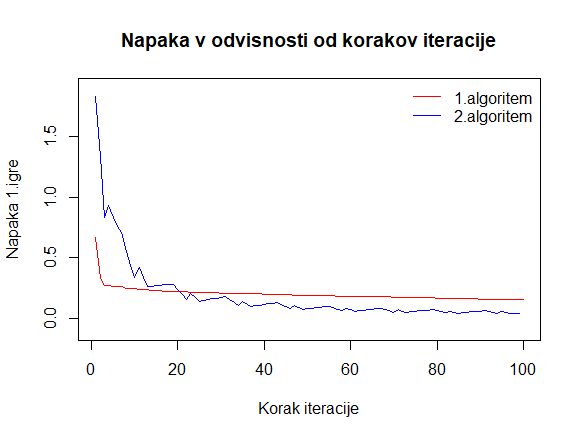
\includegraphics[width=12cm]{napaka1.png}
    \caption{Napaka algoritmov za prvo matrično igro}
    \label{fig:napaka1}
  \end{figure}

Tabela \ref{table:1igra} prikazuje konkretne vrednosti, dobljene z obema algoritmoma pri različnemu številu korakov.
Vidimo, da je časovna zahtevnost prve metode precej večja od druge; pri 15000 iteracijah prva metoda za izračun rešitve igre
porabi $5,5$-krat več časa. Pri $k = 1000$ imamo pri obeh metodah natančnost pri dveh decimalnih mestih za vse komponente. Pri $k = 15000$ prva metoda že popolnoma skonvergira
k rešitvi igre, druga metoda pa je natačna za štiri decimalna mesta.

\begin{table}[]
    \resizebox{\textwidth}{!}{\begin{tabular}{c|llll|llll|}
    \cline{2-9}
                                                                                                 & \multicolumn{4}{c|}{1. metoda}                                                                                                                       & \multicolumn{4}{c|}{2. metoda}                                                                                                                                                                                    \\ \cline{2-9} 
                                    & \multicolumn{1}{l|}{čas}    & \multicolumn{1}{l|}{v}       & \multicolumn{1}{l|}{x}                                                                   & y                                                         & \multicolumn{1}{l|}{čas}    & \multicolumn{1}{l|}{v}       & \multicolumn{1}{l|}{x}                                                                   & y                                                         \\ \hline
    \multicolumn{1}{|c|}{k =  1}    & \multicolumn{1}{l|}{0.0020} & \multicolumn{1}{l|}{3}       & \multicolumn{1}{l|}{\begin{tabular}[c]{@{}l@{}}0.33333\\ 0.33333\\ 0.33333\end{tabular}} & \begin{tabular}[c]{@{}l@{}}0\\ 1\end{tabular}             & \multicolumn{1}{l|}{0.0009} & \multicolumn{1}{l|}{1.5}  & \multicolumn{1}{l|}{\begin{tabular}[c]{@{}l@{}}0.5\\ 0.5\\ 0\end{tabular}}               & \begin{tabular}[c]{@{}l@{}}0\\ 0.5\end{tabular}           \\ \hline
    \multicolumn{1}{|c|}{k = 2}     & \multicolumn{1}{l|}{0.0020} & \multicolumn{1}{l|}{3.49020} & \multicolumn{1}{l|}{\begin{tabular}[c]{@{}l@{}}0.33333\\ 0.33333\\ 0.33333\end{tabular}} & \begin{tabular}[c]{@{}l@{}}0.5\\ 0.5\end{tabular}         & \multicolumn{1}{l|}{0.0014} & \multicolumn{1}{l|}{2}  & \multicolumn{1}{l|}{\begin{tabular}[c]{@{}l@{}}0.66667\\ 0.33333\\ 0\end{tabular}}       & \begin{tabular}[c]{@{}l@{}}0.33333\\ 0.33333\end{tabular} \\ \hline
    \multicolumn{1}{|c|}{k = 10}    & \multicolumn{1}{l|}{0.0155} & \multicolumn{1}{l|}{3.31150} & \multicolumn{1}{l|}{\begin{tabular}[c]{@{}l@{}}0.34199\\ 0.45804\\ 0.19997\end{tabular}} & \begin{tabular}[c]{@{}l@{}}0.34425\\ 0.65575\end{tabular} & \multicolumn{1}{l|}{0.0020} & \multicolumn{1}{l|}{3}  & \multicolumn{1}{l|}{\begin{tabular}[c]{@{}l@{}}0.45454\\ 0.45454\\ 0\end{tabular}}       & \begin{tabular}[c]{@{}l@{}}0.27273\\ 0.63636\end{tabular} \\ \hline
    \multicolumn{1}{|c|}{k = 50}    & \multicolumn{1}{l|}{0.0156} & \multicolumn{1}{l|}{3.33100} & \multicolumn{1}{l|}{\begin{tabular}[c]{@{}l@{}}0.47646\\ 0.40436\\ 0.11918\end{tabular}} & \begin{tabular}[c]{@{}l@{}}0.33100\\ 0.66900\end{tabular} & \multicolumn{1}{l|}{0.0030} & \multicolumn{1}{l|}{3.25490}  & \multicolumn{1}{l|}{\begin{tabular}[c]{@{}l@{}}0.64706\\ 0.33333\\ 0.01961\end{tabular}} & \begin{tabular}[c]{@{}l@{}}0.35294\\ 0.62746\end{tabular} \\ \hline
    \multicolumn{1}{|c|}{k = 100}   & \multicolumn{1}{l|}{0.0369} & \multicolumn{1}{l|}{3.33147} & \multicolumn{1}{l|}{\begin{tabular}[c]{@{}l@{}}0.51447\\ 0.39017\\ 0.09536\end{tabular}} & \begin{tabular}[c]{@{}l@{}}0.33146\\ 0.66854\end{tabular} & \multicolumn{1}{l|}{0.0049} & \multicolumn{1}{l|}{3.28713}  & \multicolumn{1}{l|}{\begin{tabular}[c]{@{}l@{}}0.66337\\ 0.32673\\ 0.00990\end{tabular}} & \begin{tabular}[c]{@{}l@{}}0.33663\\ 0.65347\end{tabular} \\ \hline
    \multicolumn{1}{|c|}{k = 500}   & \multicolumn{1}{l|}{0.0953} & \multicolumn{1}{l|}{3.33301} & \multicolumn{1}{l|}{\begin{tabular}[c]{@{}l@{}}0.64108\\ 0.34289\\ 0.01603\end{tabular}} & \begin{tabular}[c]{@{}l@{}}0.33302\\ 0.66670\end{tabular} & \multicolumn{1}{l|}{0.0156} & \multicolumn{1}{l|}{3.32335} & \multicolumn{1}{l|}{\begin{tabular}[c]{@{}l@{}}0.66467\\ 0.33333\\ 0.00200\end{tabular}} & \begin{tabular}[c]{@{}l@{}}0.33134\\ 0.66667\end{tabular} \\ \hline
    \multicolumn{1}{|c|}{k = 1000}  & \multicolumn{1}{l|}{0.1207} & \multicolumn{1}{l|}{3.33330} & \multicolumn{1}{l|}{\begin{tabular}[c]{@{}l@{}}0.66391\\ 0.33436\\ 0.00173\end{tabular}} & \begin{tabular}[c]{@{}l@{}}0.33330\\ 0.66670\end{tabular} & \multicolumn{1}{l|}{0.0312} & \multicolumn{1}{l|}{3.33290} & \multicolumn{1}{l|}{\begin{tabular}[c]{@{}l@{}}0.66633\\ 0.33257\\ 0.00010\end{tabular}} & \begin{tabular}[c]{@{}l@{}}0.33367\\ 0.66533\end{tabular} \\ \hline
    \multicolumn{1}{|c|}{k = 15000} & \multicolumn{1}{l|}{2.4360} & \multicolumn{1}{l|}{3.33333} & \multicolumn{1}{l|}{\begin{tabular}[c]{@{}l@{}}0.66667\\ 0.33333\\ 0\end{tabular}}       & \begin{tabular}[c]{@{}l@{}}0.33333\\ 0.66667\end{tabular} & \multicolumn{1}{l|}{0.4397} & \multicolumn{1}{l|}{3.33304} & \multicolumn{1}{l|}{\begin{tabular}[c]{@{}l@{}}0.66656\\ 0.33338\\ 0.00007\end{tabular}} & \begin{tabular}[c]{@{}l@{}}0.33338\\ 0.66656\end{tabular} \\ \hline
    \end{tabular}}
    \caption{Primerjava rezultatov za 1. igro}
    \label{table:1igra}
    \end{table} 
Nato si oglejmo matriko velikosti $7 \times 7$:
\begin{equation*}
\begin{bmatrix}
    0 & -1 & -2 & 0 & 0 & 2 & 1\\
    1 & 0 & 0 & 4  & 0 & 0 & -1\\
    2 & 0 & 0 & -1 & 1 & 0 & -1\\
    0 &-4 & 1 & 0 & 0 & -1 & 1\\
    0 & 0 & -1 & 0 & 0 & -3 & 1\\
    -2 & 0 & 0 & 1 & 3 & 0 & -1\\
    -1 & 1 & 1 & -1 & -1 & 1 & 0 
\end{bmatrix}
\end{equation*}

Ker je 2. matrična igra simetrična, je njena vrednost $v = 0$. Optimalni strategiji sta 
$X = [1/9, 1/9, 15/90, 5/90, 15/90, 5 / 90, 1 /3]$ in 
$Y = [1 / 9, 1 / 9, 15/90, 5 / 90, 15 / 90,  5 / 90, 1 /3]$. 
Podobno kot prej, si poglejmo graf \ref{fig:vred2}, ki prikazuje, kako hitro konvergira
 vrednost 2. igre, 
dobljena z obema metodama proti pravi vrednosti ($v = 0$). Ponovno sem zaradi boljše preglednosti
naredila le
100 korakov iteracije. Opazimo, da se vrednost igre, dobljene z drugim algoritmom, hitreje približa
pravi vrednosti igre, kar je najverjetneje povezano z izbiro začetnega približka. Zdi se, da je konvergenca hitra
pri obeh algoritmih.
\begin{figure}
    \centering
    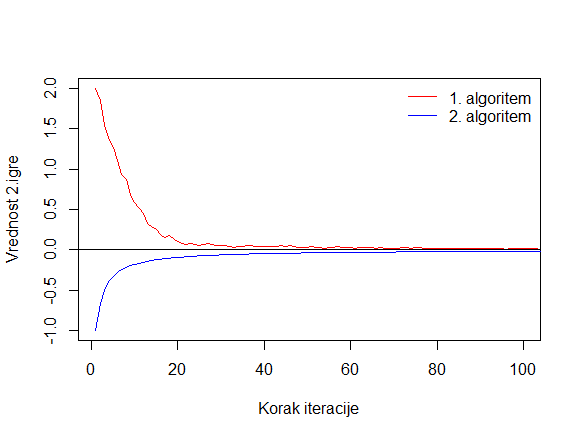
\includegraphics[width=12cm]{2igra_vrednosti.png}
    \caption{Vrednosti druge matrične igre}
    \label{fig:vred2}
  \end{figure}

Naslednji graf \ref{fig:napaka2} prikazuje, kako se spreminja napaka, dobljena pri obeh algoritmih v odvisnosti od števila iteracij. Zanimivo je, da
je situacija obratna, kot pri prvi matrični igri. Tu je konvergenca napake, dobljene s prvim algoritmom nekoliko hitrejša kot konvergenca napake, dobljene z drugim algoritmom.
  \begin{figure}
    \centering
    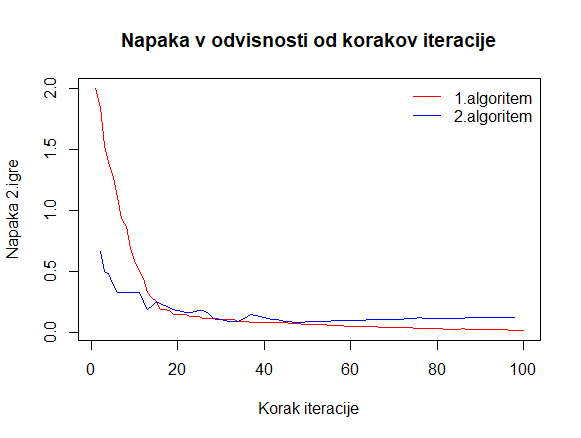
\includegraphics[width=12cm]{napaka2igra.png}
    \caption{Napaka algoritmov za prvo matrično igro}
    \label{fig:napaka2}
  \end{figure}

Podobno kot prej, tabela \ref{table:2igra} prikazuje konkretne vrednosti, dobljene z obema algoritmoma pri različnemu številu korakov. Pri $k = 500$ se prva metoda približa 
pravi rešitvi v dveh decimalnih mestih natačno pri vseh komponentah. Druga metoda konvergira
nekoliko počasneje in se pravi rešitvi ne približa v dveh decimalnih mestih niti pri $k = 15000$, medtem ko se zdi, da pri takem številu korakov, prva metoda
že popolnoma skonvergira.  Zopet je čas izvajanja algoritma daljši pri prvi metodi. 
\begin{table}[]
    \resizebox{\textwidth}{!}{\begin{tabular}{c|llll|llll|}
    \cline{2-9}
                                    & \multicolumn{4}{c|}{1. metoda}                                                                                                                                                                                                                                                                                        & \multicolumn{4}{c|}{2. metoda}                                                                                                                                                                                                                                                                                  \\ \cline{2-9} 
                                    & \multicolumn{1}{l|}{čas}     & \multicolumn{1}{l|}{v}       & \multicolumn{1}{l|}{x}                                                                                                                  & y                                                                                                             & \multicolumn{1}{l|}{čas}     & \multicolumn{1}{l|}{v}       & \multicolumn{1}{l|}{x}                                                                                                             & y                                                                                                            \\ \hline
    \multicolumn{1}{|c|}{k =  1}    & \multicolumn{1}{l|}{0.00365} & \multicolumn{1}{l|}{1.84615} & \multicolumn{1}{l|}{\begin{tabular}[c]{@{}l@{}}0.01282\\ 0.16667\\ 0.16667\\ 0\\ 0.16667\\ 0.16667\\ 0.32051\end{tabular}}              & \begin{tabular}[c]{@{}l@{}}0.14286\\ 0.14286\\ 0.14286\\ 0.14286\\ 0.14286\\ 0.14286\\ 0.14286\end{tabular}   & \multicolumn{1}{l|}{0.00165} & \multicolumn{1}{l|}{-1}    & \multicolumn{1}{l|}{\begin{tabular}[c]{@{}l@{}}0\\ 0\\ 0.5\\ 0\\ 0\\ 0\\ 0.5\end{tabular}}                                         & \begin{tabular}[c]{@{}l@{}}0.5\\ 0\\ 0\\ 0\\ 0\\ 0\\ 0\end{tabular}                                          \\ \hline
    \multicolumn{1}{|c|}{k = 2}     & \multicolumn{1}{l|}{0.00489} & \multicolumn{1}{l|}{0.73931} & \multicolumn{1}{l|}{\begin{tabular}[c]{@{}l@{}}0.21520\\ 0\\ 0\\ 0.20238\\ 0.36904\\ 0\\ 0.21337\end{tabular}}                          & \begin{tabular}[c]{@{}l@{}}0.14286\\ 0.14286\\ 0.14286\\ 0.14286\\ 0.14286\\ 0.14286\\ 0.14286\end{tabular}   & \multicolumn{1}{l|}{0.00270} & \multicolumn{1}{l|}{-0.66667} & \multicolumn{1}{l|}{\begin{tabular}[c]{@{}l@{}}0\\ 0.33333\\ 0.33333\\ 0\\ 0\\ 0\\ 0.33333\end{tabular}}                           & \begin{tabular}[c]{@{}l@{}}0.33333\\ 0\\ 0\\ 0.33333\\ 0\\ 0\\ 0\end{tabular}                                \\ \hline
    \multicolumn{1}{|c|}{k = 10}    & \multicolumn{1}{l|}{0.00319} & \multicolumn{1}{l|}{0.53636} & \multicolumn{1}{l|}{\begin{tabular}[c]{@{}l@{}}0.06687\\ 0.22339\\ 0.24321\\ 0\\ 0.21376\\ 0\\ 0.25274\end{tabular}}                    & \begin{tabular}[c]{@{}l@{}}0.14286\\ 0.14286\\ 0.14286\\ 0.14286\\ 0.14286\\ 0.14286\\ 0.14286\end{tabular}   & \multicolumn{1}{l|}{0.00575} & \multicolumn{1}{l|}{-0.18182} & \multicolumn{1}{l|}{\begin{tabular}[c]{@{}l@{}}0.18182\\ 0.27273\\ 0.09091\\ 0.09091\\ 0.27273\\ 0\\ 0.09091\end{tabular}}         & \begin{tabular}[c]{@{}l@{}}0.09091\\ 0.27273\\ 0.09091\\ 0.09091\\ 0\\ 0.36364\end{tabular}                  \\ \hline
    \multicolumn{1}{|c|}{k = 50}    & \multicolumn{1}{l|}{0.01561} & \multicolumn{1}{l|}{0.02724} & \multicolumn{1}{l|}{\begin{tabular}[c]{@{}l@{}}0.11101\\ 0.10108\\ 0.16020\\ 0.06888\\ 0.16563\\ 0.04690\\ 0.34627\end{tabular}}        & \begin{tabular}[c]{@{}l@{}}0.10855\\ 0.14050\\ 0.14894\\ 0.05297\\ 0.16978 \\ 0.11520 \\ 0.26410\end{tabular} & \multicolumn{1}{l|}{0.00418} & \multicolumn{1}{l|}{-0.03922} & \multicolumn{1}{l|}{\begin{tabular}[c]{@{}l@{}}0.11765\\ 0.09804\\ 0.27451\\ 0.07843\\ 0.07843\\ 0.03922\\ 0.31373\end{tabular}}   & \begin{tabular}[c]{@{}l@{}}0.11765\\ 0.13725\\ 0.17647\\ 0.05882\\ 0.07843\\ 0.07843\\ 0.33333\end{tabular}  \\ \hline
    \multicolumn{1}{|c|}{k = 100}   & \multicolumn{1}{l|}{0.03798} & \multicolumn{1}{l|}{0.00560} & \multicolumn{1}{l|}{\begin{tabular}[c]{@{}l@{}}0.11286\\ 0.11280\\ 0.16732\\ 0.05262\\ 0.16899\\ 0.05386\\ 0.33153\end{tabular}}        & \begin{tabular}[c]{@{}l@{}}0.11161\\ 0.13054\\ 0.14982\\ 0.05716\\ 0.16783\\ 0.07269\\ 0.31035\end{tabular}   & \multicolumn{1}{l|}{0.00557} & \multicolumn{1}{l|}{-0.01980} & \multicolumn{1}{l|}{\begin{tabular}[c]{@{}l@{}}0.10891\\ 0.09901\\ 0.15842\\ 0.03960\\ 0.17822\\ 0.08911\\ 0.32673\end{tabular}}   & \begin{tabular}[c]{@{}l@{}}0.12871\\ 0.11881\\ 0.18812\\ 0.04951\\ 0.15842\\ 0.03960 \\ 0.30693\end{tabular} \\ \hline
    \multicolumn{1}{|c|}{k = 500}   & \multicolumn{1}{l|}{0.18201} & \multicolumn{1}{l|}{0.00092} & \multicolumn{1}{l|}{\begin{tabular}[c]{@{}l@{}}0.111015\\ 0.111365\\ 0.166570\\ 0.055421\\ 0.166630\\ 0.055414\\ 0.333585\end{tabular}} & \begin{tabular}[c]{@{}l@{}}0.11136\\ 0.11839\\ 0.16141\\ 0.05547 \\ 0.16639\\ 0.05588\\ 0.33111\end{tabular}  & \multicolumn{1}{l|}{0.03899} & \multicolumn{1}{l|}{-0.00399} & \multicolumn{1}{l|}{\begin{tabular}[c]{@{}l@{}}0.09980\\ 0.14371 \\ 0.16567 \\ 0.05589\\ 0.16567\\ 0.05190\\ 0.31737\end{tabular}} & \begin{tabular}[c]{@{}l@{}}0.12575\\ 0.15369\\ 0.13573 \\ 0.04591\\ 0.14970\\ 0.06387\\ 0.32335\end{tabular} \\ \hline
    \multicolumn{1}{|c|}{k = 1000}  & \multicolumn{1}{l|}{0.30498} & \multicolumn{1}{l|}{0.00021} & \multicolumn{1}{l|}{\begin{tabular}[c]{@{}l@{}}0.111174\\ 0.111040\\ 0.166691\\ 0.055660\\ 0.166655\\ 0.055518\\ 0.333259\end{tabular}} & \begin{tabular}[c]{@{}l@{}}0.11109\\ 0.11311\\ 0.16518\\ 0.05562\\ 0.16665\\ 0.05559\\ 0.33277\end{tabular}   & \multicolumn{1}{l|}{0.04474} & \multicolumn{1}{l|}{-0.00199} & \multicolumn{1}{l|}{\begin{tabular}[c]{@{}l@{}}0.11289\\ 0.11089\\ 0.17183\\ 0.04695\\ 0.16484\\ 0.05594\\ 0.33666\end{tabular}}   & \begin{tabular}[c]{@{}l@{}}0.11588\\ 0.11189\\ 0.17083\\ 0.04595\\ 0.17383\\ 0.04895\\ 0.33167\end{tabular}  \\ \hline
    \multicolumn{1}{|c|}{k = 15000} & \multicolumn{1}{l|}{4.83584} & \multicolumn{1}{l|}{3.1e-17} & \multicolumn{1}{l|}{\begin{tabular}[c]{@{}l@{}}0.11111\\ 0.11111\\ 0.16667\\ 0.05556\\ 0.16667\\ 0.05556\\ 0.33333\end{tabular}}        & \begin{tabular}[c]{@{}l@{}}0.11111\\ 0.11111\\ 0.16667\\ 0.05556\\ 0.16667\\ 0.05556\\ 0.33333\end{tabular}   & \multicolumn{1}{l|}{0.58264} & \multicolumn{1}{l|}{-0.00013} & \multicolumn{1}{l|}{\begin{tabular}[c]{@{}l@{}}0.11312\\ 0.11112\\ 0.16732\\ 0.05466\\ 0.16299\\ 0.05520\\ 0.33558\end{tabular}}   & \begin{tabular}[c]{@{}l@{}}0.10752\\ 0.11179\\ 0.16739\\ 0.05786\\ 0.16545\\ 0.05446\\ 0.33544\end{tabular}  \\ \hline
    \end{tabular}}
    \caption{Primerjava rezultatov za 2. igro}
    \label{table:2igra}
    \end{table}


\section{Spletni vmesnik}
V datoteki \textit{spletnivmesnik.py} sem s pomočjo \textit{Bottle}-a naredila aplikacijo za izračun rešitve
matrične igre. Ta vas najprej vpraša po vaši matrični igri in nato izračuna vrednost in optimalno strategijo igre s pomočjo
linearnega programiranja in obeh zgoraj obravnavnih iterativnih metod. (Aplikacija še ni popolnoma dokončana).
\section{Zaključek}

Oba implementirana iteracijska algoritma konvergirata proti rešitvi igre, a z različno hitrostjo in časovno zahtevnostjo. \\
Drugi algoritem ima manjšo časovno zahtevnost, a rezultati kažejo na to, da je konvergenca počasnejša kot pri prvem algoritmu.
Menim, da je hitrost konvergence prve metode močno odvisna tudi od začetnega približka, kar je vsekakor vredno nadaljnjega raziskovanja.
Prav tako, pa sem opazila tudi, da oba algoritma ne izbereta vedno najbližje rešitve.

 
\begin{thebibliography}{99}
\bibitem{vir1}
    J.~Robinson, \emph{An Iterative Method of Solving a Game},  Annals of Mathematics, \textbf{1951}  strani od 296 do 301. Dostopno na: https://www.jstor.org/stable/1969530
\bibitem{vir2}
  R. J.~Jirka, \emph{An iterative method for finding a solution to a zero-sum two person rectangular game}, \textbf{1959}.
\end{thebibliography}
    \end{document}
